\chapter{Аутентификация пользователя}
\selectlanguage{russian}

\section{Многофакторная аутентификация}

Для защищённых приложений применяется \emph{многофакторная} аутентификация одновременно по факторам различной природы:
\begin{enumerate}
    \item Свойство, которым обладает субъект. Например: биометрия, природные уникальные отличия (лицо, радужная оболочка глаз, папиллярные узоры, последовательность ДНК).
    \item Знание -- информация, которую знает субъект. Например: пароль, PIN (Personal Identification Number).
    \item Владение -- вещь, которой обладает субъект. Например: электронная или магнитная карта, флэш-память.
%    \item Факторы присвоения. Например, номер машины, RFID-метка.
\end{enumerate}

В обычных массовых приложениях из-за удобства использования применяется аутентификация только по \emph{паролю}\index{пароль}, который является общим секретом пользователя и информационной системы. Биометрическая аутентификация по отпечаткам пальцев применяется существенно реже. Как правило, аутентификация по отпечаткам пальцев является дополнительным, а не вторым обязательным фактором (тоже из-за удобства её использования).

%Так же явно или неявно используется аутентификация по факторам:
%\begin{enumerate}
%    \item Социальная сеть. Доверие к индивидууму в личном или интернет общении, на основании общих связей.
%    \item Географическое положение. Например, для проверки оплаты товаров по кредитной карте.
%    \item Время. Доступ к сервисам или местам только в определённое время.
%    \item И др.
%\end{enumerate}


\section[Энтропия и криптостойкость паролей]{Энтропия и криптостойкость \protect\\ паролей}

Стандартный набор символов паролей, которые можно набрать на клавиатуре, используя английские буквы и небуквенные символы, состоит из $D=94$ символов. При длине пароля $L$ символов и предположении равновероятного использования символов энтропия паролей равна
    \[ H = L \log_2 D. \]

Клод Шеннон (\langen{Claude Elwood Shannon}), исследуя энтропию символов английского текста, изучал вероятность успешного предсказания людьми следующего символа по первым нескольким символам слов или текста. В результате Шеннон получил оценку энтропии первого символа $s_1$ текста порядка $H(s_1) \approx 4{,}6$--$4{,}7$ бит/символ и оценки энтропий последующих символов, постепенно уменьшающиеся до $H(s_9) \approx 1{,}5$ бит/символ для 9-го символа. Энтропия для длинных текстов художественных произведений получила оценку $H(s_\infty) \approx 0{,}4$ бит/символ.

Статистические исследования баз паролей показывают, что в англоязычных текстах наиболее часто используются буквы <<a>>, <<e>>, <<o>>, <<r>> и цифра <<1>>.

NIST (Национальный институт стандартов и технологий США, \langen{National Institute of Standards and Technology})  использует следующие рекомендации для оценки энтропии паролей\index{энтропия!пароля}, создаваемых людьми.
\begin{enumerate}
    \item Энтропия первого символа $H(s_1) = 4$ бит/символ.
    \item Энтропия со 2-го по 8-й символы $H(s_{i}) = 2$ бит/символ, $2 \leq i \leq 8$.
    \item Энтропия с 9-го по 20-й символы $H(s_{i}) = 1{,}5$ бит/символ, $9 \leq i \leq 20$.
    \item Энтропия с 21-го символа $H(s_{i}) = 1$ бит/символ, $i \geq 21$.
    \item Проверка композиции на использование символов разных регистров и небуквенных символов добавляет до 6-ти бит энтропии пароля.
    \item Словарная проверка на слова и часто используемые пароли добавляет до 6 бит энтропии для коротких паролей. Для 20-символьных и более длинных паролей прибавка к энтропии -- 0 бит.
\end{enumerate}

Для оценки энтропии пароля нужно сложить энтропии символов $H(s_i)$ и сделать дополнительные надбавки, если пароль удовлетворяет тестам на композицию и отсутствует в словаре.

\begin{table}[!ht]
    \caption{Оценка NIST предполагаемой энтропии паролей\label{tab:password-entropy}}
    \centering
    {\renewcommand{\arraystretch}{1.25}
    \begin{tabular}{|c|c|c|c|c|}
        \hline
            \multirow{2}{*}{\parbox{1.5cm}{\medskip\medskip\medskip \centering {\footnotesize Длина пароля, символы}}} &
            \multicolumn{3}{c|}{\parbox{4.5cm}{\medskip \centering {\footnotesize Энтропия паролей пользователей по критериям NIST}}} &
            \multirow{2}{*}{\parbox{2cm}{\centering {\footnotesize \medskip\medskip Энтропия случайных равновероятных паролей}}} \\ [3.5ex]
        \cline{2-4}
            &
            \parbox{1.5cm}{\centering {\footnotesize \medskip\medskip Без проверок}} &
            \parbox{1.5cm}{\centering {\footnotesize \medskip\medskip Словарная проверка}} &
            \parbox{1.5cm}{\centering {\tiny \medskip Словарная и композиционная проверка}} &
            \\ [4ex]
        \hline
        4  & 10 & 14 & 16 & 26.3 \\
        6  & 14 & 20 & 23 & 39.5 \\
        8  & 18 & 24 & 30 & 52.7 \\
        10 & 21 & 26 & 32 & 65.9 \\
        12 & 24 & 28 & 34 & 79.0 \\
        16 & 30 & 32 & 38 & 105.4 \\
        20 & 36 & 36 & 42 & 131.7 \\
        24 & 40 & 40 & 46 & 158.0 \\
        30 & 46 & 46 & 52 & 197.2 \\
        40 & 56 & 56 & 62 & 263.4 \\
        \hline
    \end{tabular}
    }
\end{table}

В таблице~\ref{tab:password-entropy} приведена оценка NIST на величину энтропии пользовательских паролей в зависимости от их длины, и приведено сравнение с энтропией случайных паролей с равномерным распределением символов из набора в $D=94$ символов клавиатуры. Вероятное число попыток для подбора пароля составляет $O(2^H)$. Из таблицы видно, что по критериям NIST энтропия реальных паролей в 2--4 раза меньше энтропии случайных паролей с равномерным распределением символов.

\example
Оценим общее количество существующих паролей. Население Земли -- 7 млрд. Предположим, что всё население использует компьютеры и Интернет, и у каждого человека по 10 паролей. Общее количество существующих паролей -- $7 \cdot 10^{10} \approx 2^{36}$.

Имея доступ к наиболее массовым интернет-сервисам с количеством пользователей десятки и сотни миллионов, в которых пароли часто хранятся в открытом виде из-за необходимости обновления ПО и, в частности, выполнения аутентификации, мы:
\begin{enumerate}
	\item имеем базу паролей существенной части пользователей сети Интернет; 
	\item можем статистически построить правила генерирования паролей.
\end{enumerate}

Даже если пароль хранится в защищённом виде, то при вводе, как правило, он в открытом для сервиса виде пересылается по Интернету, и все преобразования пароля для аутентификации осуществляет интернет-сервис, а не веб-браузер. Следовательно, интернет-сервис периодически имеет доступ к исходному паролю.
\exampleend

В 2002 г. был подобран ключ для 64-битного блочного шифра RC5 сетью персональных компьютеров \texttt{distributed.net}, выполнявших вычисления в фоновом режиме. Суммарное время вычислений всех компьютеров -- 1757 дней, было проверено 83\% пространства всех ключей. Это означает, что пароли с оценочной энтропией менее 64 бит, то есть \emph{все пароли} до 40 символов по критериям NIST, могут быть подобраны в настоящее время. Конечно, с оговорками на то, что 1) нет ограничений на количество и частоту попыток аутентификаций, 2) алгоритм генерации вероятных паролей эффективен.

Строго говоря, использование даже 40-символьного пароля для аутентификации или в качестве ключа блочного шифрования является небезопасным.


\subsubsection{Число паролей}

Приведём различные оценки числа паролей, выбираемых людьми. Чаще всего такие пароли основаны на словах или закономерностях естественного языка. В английском языке всего около $1\ 000\ 000 \approx 2^{20}$ слов, включая термины.

%http://www.springerlink.com/content/bh216312577r6w64/fulltext.pdf
%http://www.antimoon.com/forum/2004/4797.htm

Используемые слоги английского языка имеют вид V, CV, VC, CVV, VCC, CVC, CCV, CVCC, CVCCC, CCVCC, CCCVCC, где C -- согласная (consonant), V -- гласная (vowel). 70\% слогов имеют структуру VC или CVC. Общее число слогов $S = 8000 \dots 12000$. Средняя длина слога -- 3 буквы.

Предполагая равновероятное распределение слогов английского языка, для числа паролей из $r$ слогов получим верхнюю оценку
    \[ N_1 = S^r = 2^{13 r} \approx 2^{4.3 L_1}. \]
Средняя длина паролей составит:
    \[ L_1 \approx 3 r. \]

Теперь предположим, что пароли могут состоять только из 2--3 буквенных слогов вида CV, VC, CVV, VCC, CVC, CCV с равновероятным распределением символов. Подсчитаем число паролей $N_2$, которые могут быть построены из $r$ таких слогов. В английском алфавите число гласных букв $n_v = 10$, согласных $n_c = 16$, $n = n_v + n_c = 26$. Верхняя оценка числа $r$-слоговых паролей:
    \[ N_2 = (n_c n_v + n_v n_c + n_c n_v n_v + n_v n_c n_c + n_c n_v n_c + n_c n_c n_v)^r \approx \]
        \[ \approx \left( n_c n_v(3 n_c + n_v) \right)^r, \]
    \[ N_2 \approx \left( \frac{n^3}{2} \right)^r \approx 2^{13 r} \approx 2^{4.3 L_2}. \]
Средняя длина паролей:
    \[ L_2 = \frac{n_c n_v(2 + 2 + 3 n_v + 3 n_c + 3 n_c + 3 n_c)}{n_c n_v (1 + 1 + n_v + n_c + n_c + n_c)} \cdot r \approx 3 r. \]

Как видно, в обоих предположениях получились одинаковые оценки для числа и длины паролей.

Подсчитаем верхние оценки числа паролей из $L$ символов, предполагая равномерное распределение символов из алфавита мощностью $D$ символов: a) $D_1 = 26$ строчных букв, б) все $D_2 = 94$ печатных символа клавиатуры (латиница и небуквенные символы):
    \[ N_3 = D_1^L \approx 2^{4.7 L}, \]
    \[ N_4 = D_2^L \approx 2^{6.6 L}. \]

\begin{table}
    \caption{Различные верхние оценки числа паролей\label{tab:password-number}}
    \centering
    {\renewcommand{\arraystretch}{1.25}
    \begin{tabular}{|c|c|c|c|}
        \hline
            \multirow{2}{*}{\parbox{1.5cm}{\footnotesize\centering\medskip\medskip\medskip Длина пароля}} &
            \multicolumn{3}{c|}{\footnotesize Число паролей}
            \\
        \cline{2-4}
            &
            \parbox{2cm}{\footnotesize\centering\medskip На основе слоговой композиции} &
            \parbox{2cm}{\footnotesize\centering\medskip Алфавит $D=26$ символов} &
            \parbox{2cm}{\footnotesize\centering\medskip Алфавит $D=94$ символа}
            \\ [3.5ex]
        \hline
        6  & $2^{26}$ & $2^{28}$ & $2^{39}$ \\
        9  & $2^{39}$ & $2^{42}$ & $2^{59}$ \\
        12 & $2^{52}$ & $2^{56}$ & $2^{79}$ \\
        15 & $2^{65}$ & $2^{71}$ & $2^{98}$ \\
        21 & $2^{91}$ & $2^{99}$ & $2^{137}$ \\
        39 & $2^{169}$ & $2^{183}$ & $2^{256}$ \\
        \hline
    \end{tabular}
    }
\end{table}

Из таблицы~\ref{tab:password-number} видно, что при доступном объёме вычислений в $2^{60}$\,--\,$2^{70}$ операций, пароли вплоть до 15-ти символов, построенные на словах, слогах, изменениях слов, вставках цифр, небольшом изменении регистров и других простейших модификациях, в настоящее время могут быть найдены полным перебором как на вычислительном кластере, так и на персональном компьютере.

Для достижения криптостойкости паролей, сравнимой со 128- или 256-битовым секретным ключом, требуется выбирать пароль из 20 и 40 символов соответственно, что, как правило, не реализуется из-за сложности запоминания и возможных ошибок при вводе.


%Подсчитаем число паролей $N_1$, которые могут могут построены из $r$ ~ 2-3 буквенных слогов: $cv, vc, ccv, cvc, vcc$, где $c$ -- согласная, $v$ -- гласная. В английском алфавите $n_v = 10, n_c = 16, n = n_v + n_c = 26$. Число паролей
%    \[ N_1 = \left( n_v n_c (1 + 1 + n_c + n_c + n_c) \right)^r \approx 3^r n_v^r n_c^{2r}. \]
%Средняя длина паролей
%    \[ L = r \left( \frac{2 + 2 + 3 n_c + 3 n_c + 3 n_c}{1 + 1 + n_c + n_c + n_c} \right) \approx 3r. \]
%
%%Учтем, что $b \leq r$ символов могут быть заглавными: $N_1 \rightarrow N_2 < N_1 \binom{L}{b} \left( \frac{n}{n_v} \right)^b$. Вставим $d$ цифр в случайные места: $N_2 \rightarrow N_3 = N_2 (10 (1 + L))^d \approx N_2 (10 L)^d$.
%%
%%Общее число паролей
%%    \[ N = N_3 = 3^r 10^r 16^{2r} \binom{3r}{b} 2.6^b \left(10 \cdot 3 r \right)^d. \]
%%
%%\begin{table}[!ht]
%%    \centering
%%    \small
%%    \begin{tabular}{|c|c|c|c|c||cr|}
%%        \hline
%%        \parbox{1.3cm}{Слогов, $r$} & \parbox{1.8cm}{Заглавных букв, $b$} & \parbox{1.5cm}{Вставок цифр, $d$} & \parbox{2.8cm}{Средняя длина пароля, $L+d$} & \parbox{3cm}{Верхняя оценка числа паролей $N$} & \multicolumn{2}{|c|}{\parbox{3.2cm}{Число всех паролей}} \\
%%        \hline
%%        $2$ & $0$ & $0$ & $6$ & $2^{26}$ & $2^{36}$ & a-z \\
%%        $2$ & $2$ & $0$ & $6$ & $2^{32}$ & $2^{48}$ & A-Z, a-z \\
%%        $2$ & $2$ & $2$ & $8$ & $2^{45}$ & $2^{48}$ & A-Z, a-z, 0-9 \\
%%        \hline
%%        $3$ & $0$ & $0$ & $9$ & $2^{39}$ & $2^{54}$ & a-z \\
%%        $3$ & $3$ & $0$ & $9$ & $2^{49}$ & $2^{54}$ & A-Z, a-z \\
%%        $3$ & $3$ & $2$ & $11$ & $2^{63}$ & $2^{65}$ & A-Z, a-z, 0-9 \\
%%        \hline
%%        $4$ & $0$ & $0$ & $12$ & $2^{52}$ & $2^{93}$ & a-z \\
%%        $4$ & $3$ & $0$ & $12$ & $2^{64}$ & $2^{186}$ & A-Z, a-z \\
%%        $4$ & $3$ & $2$ & $14$ & $2^{78}$ & $2^{222}$ & A-Z, a-z, 0-9 \\
%%        \hline
%%    \end{tabular}
%%    \caption{Сравнение верхней оценки числа паролей, построенных на слогах, со всем доступным множеством паролей.}
%%    \label{tab:password-number}
%%\end{table}
%
%Учтем, что $b$ символов в пароле могут быть взяты не из 26-символьного алфавита строчных букв, а из всего алфавита в $D=94$ печатных символа клавиатуры (латиница и небуквенные символы):
%\[
%    \begin{array}{ll}
%    b=1 & N_1 \rightarrow N_2 = \frac{n_v}{n_v+n_c} 3^r n_v^{r-1} n_c^{2r} \cdot L. \]
%
%    \[ N_1 \rightarrow N_2 < N_1 \binom{L}{b} \left( \frac{D}{n_v} \right)^b. \]
%
%
%
%Общее число паролей
%    \[ N < 3^r n_v^r n_c^{2r} \binom{L}{b} \left( \frac{D}{n_v} \right)^b = 3^r 10^r 16^{2r} \binom{3r}{b} \left( \frac{94}{10} \right)^b. \]
%
%\begin{table}[!ht]
%    \centering
%    \small
%    \begin{tabular}{|c|c|c|c||cr|}
%        \hline
%        \parbox{1.5cm}{Слогов, $r$} & \parbox{3cm}{Средняя длина пароля, $L$} & \parbox{3cm}{Символов из всего алфавита, $b$} & \parbox{3cm}{Верхняя оценка числа паролей $N$} & \multicolumn{2}{|c|}{\parbox{3.2cm}{Число всех паролей, $D^L$}} \\
%        \hline
%        \multirow{3}{*}{2} & \multirow{3}{*}{6} & $0$ & $2^{26}$ & $2^{28}$ & a-z \\
%        & & $1$ & $2^{32}$ & $2^{34}$ & A-Z, a-z \\
%        & & $3$ & $2^{40}$ & $2^{39}$ & Весь алфавит \\
%        \hline
%        \multirow{3}{*}{3} & \multirow{3}{*}{9} & $0$ & $2^{39}$ & $2^{42}$ & a-z \\
%        & & $2$ & $2^{50}$ & $2^{51}$ & A-Z, a-z \\
%        & & $4$ & $2^{59}$ & $2^{59}$ & Весь алфавит \\
%        \hline
%        \multirow{3}{*}{4} & \multirow{3}{*}{12} & $0$ & $2^{52}$ & $2^{56}$ & a-z \\
%        & & $3$ & $2^{69}$ & $2^{68}$ & A-Z, a-z \\
%        & & $6$ & $2^{81}$ & $2^{77}$ & Весь алфавит \\
%        \hline
%    \end{tabular}
%    \caption{Сравнение верхней оценки числа паролей, построенных на слогах, со всем доступным множеством паролей в алфавите из $D$ символов.}
%    \label{tab:password-number}
%\end{table}
%
%Из таблицы~\ref{tab:password-number} видно, что при доступном объёме вычислений в $2^{60 \ldots 70}$ операций, пароли вплоть до 12 символов, построенные на словах, слогах, изменениях слов, вставках цифр, небольшого изменения регистров и другой простейшей обфускации, могут быть найдены перебором на кластере (или ПК) в настоящее время.


\subsubsection{Атака для подбора паролей и ключей шифрования}

В схемах аутентификации по паролю иногда используется хеширование и хранение хеша пароля на сервере. В таких случаях применима словарная атака или атака с применением заранее вычисленных таблиц для ускорения поиска.

Для нахождения пароля, прообраза хеш-функции, или для нахождения ключа блочного шифрования по атаке с выбранным шифртекстом (для одного и того же известного открытого текста и соответствующего шифртекста) может быть применён метод перебора с балансом между памятью и временем вычислений. Самый быстрый метод радужных таблиц\index{радужные таблицы} (\langen{rainbow tables}, 2003~г., \cite{Oechslin:2003}) заранее вычисляет следующие цепочки и хранит результат в памяти.

Для нахождения пароля, прообраза хеш-функции $H$, цепочка строится как
    \[ M_0 \xrightarrow{H(M_0)} h_0 \xrightarrow{R_0(h_0)} M_1 \ldots M_t \xrightarrow{H(M_t)} h_t \xrightarrow{R_t(h_t)} M_{t+1}, \]
где $R_i(h)$ -- функция редуцирования, преобразования хеша в пароль для следующего хеширования.

Для нахождения ключа блочного шифрования для одного и того же известного открытого текста $M$ таблица строится как
    \[ K_0 \xrightarrow{E_{K_0}(M)} c_0 \xrightarrow{R_0(c_0)} K_1 \ldots K_t \xrightarrow{E_{K_t}(M)} c_t \xrightarrow{R_t(c_t)} K_{t+1}, \]
где $R_i(c)$ -- функция редуцирования, преобразования шифртекста в новый ключ.

Функция редуцирования $R_i$ зависит от номера итерации, чтобы избежать дублирующихся подцепочек, которые возникают в случае коллизий между значениями в разных цепочках в разных итерациях, если $R$ постоянна. Радужная таблица размера $(m \times 2)$ состоит из строк $(M_{0,j}, M_{t+1,j})$ или $(K_{0,j}, K_{t+1,j})$, вычисленных для разных значений стартовых паролей $M_{0,j}$ или $K_{0,j}$ соответственно.

Опишем атаку на примере нахождения прообраза $\overline{M}$ хеша $\overline{h} = H(\overline{M})$. На первой итерации исходный хеш $\overline{h}$ редуцируется в сообщение $\overline{h} \xrightarrow{R_t(\overline{h})} \overline{M}_{t+1} $ и сравнивается со всеми значениями последнего столбца $M_{t+1,j}$ таблицы. Если нет совпадения, переходим ко второй итерации. Хеш $\overline{h}$ дважды редуцируется в сообщение $\overline{h} \xrightarrow{R_{t-1}(\overline{h})} \overline{M}_t \xrightarrow{H(\overline{M}_t)} \overline{h}_t \xrightarrow{R_t(\overline{h}_t)} \overline{M}_{t+1}$ и сравнивается со всеми значениями последнего столбца $M_{t+1,j}$ таблицы. Если не совпало, то переходим к третьей итерации и~т.\,д. Если для $r$-кратного редуцирования сообщение $\overline{M}_{t+1}$ содержится в таблице во втором столбце, то из совпавшей строки берётся $M_{0,j}$, и вся цепочка пробегается заново для поиска искомого сообщения $\overline{M}: ~ \overline{h} = H(\overline{M})$.

Найдём вероятность нахождения пароля в таблице. Пусть мощность множества всех паролей равна $N$. Изначально в столбце $M_{0,j}$ содержится $m_0 = m$ различных паролей. Предполагая наличие случайного отображения с пересечениями паролей $M_{0,j} \rightarrow M_{1,j}$, в $M_{1,j}$ будет $m_1$ различных паролей. Согласно задаче о размещении,
\[
    m_{i+1} = N \left( 1 - \left( 1 - \frac{1}{N} \right)^{m_i} \right) \approx N \left( 1 - e^{-\frac{m_i}{N}} \right).
\]
Вероятность нахождения пароля:
\[
    P = 1 - \prod \limits_{i=1}^t \left( 1 - \frac{m_i}{N} \right).
\]

Чем больше таблица из $m$ строк, тем больше шансов найти пароль или ключ, выполнив в наихудшем случае   $O \left( m \frac{t(t+1)}{2} \right)$ операций.

Примеры применения атаки на хеш-функциях $\textrm{MD5}$\index{хеш-функция!MD5}, $\textrm{LM}$ (т.~е. $\textrm{DES}_{\textrm{Password}} (\textrm{const})$) приведены в таблице~\ref{tab:rainbow-tables}.

\begin{table}[!ht]
    \centering
    \caption{Атаки на радужных таблицах на \emph{одном} ПК\label{tab:rainbow-tables}}
    \resizebox{\textwidth}{!}{ \begin{tabular}{|c|c|c|c|c|c|c|}
        \hline
            \multirow{2}{*}{\parbox{1cm}{\centering\footnotesize \medskip\medskip\medskip Длина, биты}} & \multicolumn{3}{c|}{\footnotesize Пароль или ключ} &
            \multicolumn{3}{c|}{\footnotesize Радужная таблица} \\
        \cline{2-7}
            &
            \parbox{1.0cm}{\centering\footnotesize Длина,\\ симв.} &
            {\footnotesize Множество} &
            {\footnotesize Мощность} &
            {\footnotesize Объём} &
            \parbox{1.7cm}{\centering\footnotesize \medspace Время вычисления таблиц} & \parbox{1.1cm}{\centering\footnotesize Время поиска} \\ [2ex]
        \hline \hline
        \multicolumn{7}{|c|}{\footnotesize Хеш LM} \\
        \hline
        &  & A--Z & $2^{33}$ & 610 MB & \multirow{3}{*}{\parbox{1.7cm}{\centering несколько лет}} & 6 с \\
        $2 \times 56$ & 14 & A--Z, 0-9 & $2^{36}$ & 3 GB &  & 15 с \\
        & & все & $2^{43}$ & 64 GB &  & 7 мин \\
        \hline \hline
        \multicolumn{7}{|c|}{\footnotesize Хеш MD5} \\
        \hline
        \rule{0pt}{2.5ex} 128 & 8 & A-Z, 0-9 & $2^{41}$ & 36 GiB & - & 4 мин \\
        \hline
    \end{tabular} }
\end{table}

\section{Аутентификация по паролю}

Из-за малой энтропии пользовательских паролей во всех системах регистрации и аутентификации пользователей применяется специальная политика безопасности. Типичные минимальные требования:
\begin{enumerate}
    \item Длина пароля от 8 символов. Использование разных регистров и небуквенных символов в паролях. Запрет паролей из словаря или часто используемых паролей. Запрет паролей в виде дат, номеров машин и других номеров.
    \item Ограниченное время действия пароля. Обязательная смена пароля по истечении срока действия.
    \item Блокирование возможности аутентификации после нескольких неудачных попыток. Ограниченное число актов аутентификации в единицу времени. Временная задержка перед выдачей результата аутентификации.
\end{enumerate}

Дополнительные меры предосторожности для пользователей:
\begin{enumerate}
    \item Не использовать одинаковые или похожие пароли для разных систем, таких как электронная почта, вход в ОС, электронная платёжная система, форумы, социальные сети. Пароль часто передаётся в открытом виде по сети. Пароль доступен администратору системы, возможны утечки конфиденциальной информации с серверов. Поэтому следует стараться выбирать случайные стойкие пароли.
    \item Не записывать пароли. Никому не сообщать пароль, даже администратору. Не передавать пароли по почте, телефону, Интернету и~т.\,д.
    \item Не использовать одну и ту же учётную запись для разных пользователей, даже в виде исключения.
    \item Всегда блокировать компьютер, когда пользователь отлучается от него, даже на короткое время.
\end{enumerate}

\section[Пароли и аутентификация в ОС]{Хранение паролей и \protect\\ аутентификация в ОС}
\selectlanguage{russian}

Для усложнения подбора пароля и защиты от словарной атаки перед процедурой хэширования к паролю добавляется <<соль>> -- случайная битовая строка. \emph{<<Солью>>} (salt)\index{соль} называется (псевдо)случайная битовая строка $s$, добавляемая к аргументу $m$ (паролю) функции хэширования $h(m)$ для рандомизации хэширования одинаковых сообщений.

\emph{Словарная} атака заключается в том, что злоумышленник один раз заранее вычисляет таблицы хэшей от наиболее \emph{вероятных} сообщений, то есть составляет словарь пароль-хэш, и далее производит поиск по вычисленной таблице для взламывания исходного сообщения. Ранее словарные атаки использовались для взлома паролей $m$, которые хранились в виде обычных хэшей $h(m)$. Усовершенствованной словарной атакой является метод радужных таблиц, позволяющий практически взламывать хэши длиной до 64--128 бит. Использование <<соли>> делает невозможной словарную атаку, так как значение функции вычисляется уже не от оригинального пароля, а от конкатенации <<соли>> и пароля.

<<Соль>> может храниться как отдельное значение, единственное и уникальное для системы целиком, так и быть уникальной для каждого сохранённого пароля и храниться со значением функции хэширования:
\begin{itemize}
	\item $s ~\|~ h(s ~\|~ m)$;
	\item $s ~\|~ h(m ~\|~ s)$;
	\item $s_1 ~\|~ h(m ~\|~ s_1 ~\|~ s_2)$.
\end{itemize}

В первом случае функция хэширования вычисляется от конкатенации (склеивания) <<соли>> и пароля пользователя. Во втором случае в строке сначала идёт пароль, а потом -- <<соль>>. Это позволяет немного усложнить задачу злоумышленнику при переборе паролей (он не сможет сократить время вычисления значения функции хэширования за счёт одинакового префикса у всех аргументов функции хэширования). В третьем случае используется сразу две <<соли>>: одна хранится вместе с паролем, а вторая выступает внешним параметром, хранящимся отдельно от базы данных паролей.

В рассмотренной ранее модели построения паролей в виде слогов с элементами небольшой модификации мы получили количество паролей около $2^{70}$ для 12-символьных паролей. Данный объём вычислений уже почти достижим. Следовательно, даже <<соль>> не защищает пароли от взлома, если у злоумышленника есть доступ к файлу с паролями или возможность неограниченных попыток аутентификации. Поэтому файлы с паролями дополнительно защищаются, а в системы аутентификации по паролю вводят ограничения на неуспешные попытки аутентификации.

\subsection[Unix]{Хранение паролей в Unix}

В ОС Unix пароль $m$ пользователя хранится в файле \texttt{/etc/shadow} в виде хэша (SHA, MD5 и~т.~д.) или результата шифрования (DES, Blowfish и~т.~д.), вычисленного с <<солью>> $s$ длиной от 2 (для функции crypt в оригинальной ОС UNIX) до 16 (для Blowfish в OpenBSD) ASCII-символов. То, как используется <<соль>>, зависит от используемого алгоритма. Например, в традиционном алгоритме, используемом в оригинальном UNIX, <<соль>> модифицирует s-блоки и p-блоки в протоколе DES.

Файл \texttt{/etc/shadow} доступен только привилегированным процессам, что вносит дополнительную защиту.


\subsection[Windows]{Хранение паролей и аутентификация в \protect\\ Windows}

%[MS-NLMP]: NT LAN Manager (NTLM) Authentication Protocol Specification -- 09/25/2009, Rev. 11.0
%http://blogs.technet.com/authentication/archive/2006/04/07/ntlm-s-time-has-passed.aspx
%http://technet.microsoft.com/en-us/library/cc755284(WS.10).aspx -- Windows Authentication, Updated: February 7, 2008
%http://207.46.16.252/en-us/magazine/2006.08.securitywatch.aspx - The Most Misunderstood Windows Security Setting of All Time, Jesper Johansson
%http://en.wikipedia.org/wiki/NTLM
%http://www.windowsnetworking.com/nt/atips/atips92.shtml

ОС Windows, начиная с Vista, Server 2008, Windows 7, сохраняет пароли в виде NT-хэша, который вычисляется как 128-битовый хэш MD4 от пароля в Unicode кодировке. NT-хэш не использует <<соль>>, поэтому применима словарная атака. На словарной атаке основаны программы поиска (взлома) паролей для Windows. Файл паролей называется SAM (\langen{Security Account Manager}) в случае локальной аутентификации. Если пароли хранятся на сетевом сервере, то они хранятся в специальном файле, доступ к которому ограничен.

В последнем протоколе аутентификации NTLMv2\index{протокол!NTLM}\index{протокол!NTLMv2}~\cite{MS-NLMP} пользователь для входа в свой компьютер аутентифицируется либо локально на компьютере, либо удалённым сервером, если учётная запись пользователя хранится на сервере. Пользователь с именем $user$ вводит пароль в программу-\emph{клиент}, которая, взаимодействуя с программой-\emph{сервером} (локальной или удалённой на сервере домена $domain$), аутентифицирует пользователя для входа в систему.
\begin{enumerate}
    \item Клиент $\rightarrow$ Сервер: запрос аутентификации.
    \item Клиент $\leftarrow$ Сервер: 64-битовая псевдослучайная одноразовая метка $n_s$.
    \item Вводимый пользователем пароль хэшируется в $\textrm{NThash}$ без <<соли>>. Клиент генерирует 64-битовую псевдослучайную одноразовую метку $n_c$, создаёт метку времени $ts$. Далее вычисляются 128-битовые имитовставки\index{имитовставка} $\HMAC$ на хэш-функции MD5 с ключами $\textrm{NT-hash}$ и $\textrm{NTOWF}$:
        \[ \textrm{NThash} = \text{MD4}(\text{Unicode}(\text{пароль})), \]
        \[ \textrm{NTOWF} = \textrm{HMAC-MD5}_{\textrm{NThash}}(user, domain), \]
        %\[ \text{LMv2-response} = \text{HMAC-MD5}_{\text{NTLMv2-hash}}(n_c, n_s), \]
        \[ \textrm{NTLMv2-response} = \textrm{HMAC-MD5}_{\textrm{NTOWF}}(n_c, n_s, ts, domain). \]
    \item Клиент $\rightarrow$ Сервер: $(n_c, \textrm{NTLMv2-response})$. %LMv2-response,
    \item Сервер для указанных имён пользователя и домена извлекает из базы паролей требуемый NT-hash, производит аналогичные вычисления и сравнивает значения имитовставок. Если они совпадают, аутентификация успешна.
\end{enumerate}

В случае аутентификации на локальном компьютере сравниваются значения $\textrm{NTOWF}$: вычисленные от пароля пользователя и извлечённые из файла паролей SAM.

Как видно, протокол аутентификации NTLMv2 обеспечивает одностороннюю аутентификацию пользователя серверу (или своему ПК).

При удалённой аутентификации по сети последние версии Windows используют протокол Kerberos, который обеспечивает взаимную аутентификацию, и, только если аутентификация по Kerberos не поддерживается клиентом или сервером, она происходит по NTLMv2.


\section{Аутентификация в веб-сервисах}
\selectlanguage{russian}

В настоящий момент HTTP\index{протокол!HTTP} (вместе с HTTPS\index{протокол!HTTPS}) является основным протоколом, используемым в сети Интернет для доступа к веб-сервисам (например к социальным сетям или веб-клиентам электронной почты). Данный протокол является протоколом типа <<запрос-ответ>>\index{протокол!запрос-ответ}, причём для каждого запроса открывается новое соединение с сервером\footnote{Для версии протокола HTTP/1.0 существует неофициальное~\cite[p.~17]{Totty:2002} расширение в виде заголовка \texttt{Connection: Keep-Alive}, который позволяет использовать одно соединение для нескольких запросов. Версия протокола HTTP/1.1 по умолчанию~\cite[6.3.~Persistence]{rfc7230} устанавливает поддержку выполнения нескольких запросов в рамках одного соединения. Однако все запросы всё равно выполняются независимо друг от друга.}. То есть протокол HTTP не является сессионным протоколом\index{протокол!сессионный}. В связи с этим задачу аутентификации на веб-сервисах можно разделить на задачи первичной и вторичной аутентификаций. \emph{Первичной аутентификацией}\index{аутентификация!первичная} будем называть механизм обычной аутентификации пользователя в рамках некоторого HTTP-запроса, а \emph{вторичной}\index{аутентификация!вторичная} (или \emph{повторной}\index{аутентификация!повторная}) -- некоторый механизм подтверждения в рамках последующих HTTP-запросов, что пользователь уже был \emph{ранее} аутентифицирован веб-сервисом в рамках первичной аутентификации.

Аутентификация в веб-сервисах также бывает \emph{односторонней}\index{аутентификация!односторонняя} (как со стороны клиента, так и со стороны сервиса) и \emph{взаимной}\index{аутентификация!взаимная}. Под аутентификацией веб-сервиса обычно понимается возможность сервиса доказать клиенту, что он является именно тем веб-сервисом, к которому хочет получить доступ пользователь, а не его мошеннической подменой, созданной злоумышленниками. Для аутентификации веб-сервисов используется механизм сертификатов открытых ключей\index{сертификат открытого ключа} протокола HTTPS\index{протокол!HTTPS} с использованием инфраструктуры открытых ключей\index{инфраструктура открытых ключей} (см. раздел~\ref{chapter-public-key-infrastructure}).

При использовании протокола HTTPS\index{протокол!HTTPS} и наличии соответствующей поддержки со стороны веб-сервиса клиент также имеет возможность аутентифицировать себя с помощью своего сертификата открытого ключа\index{сертификат открытого ключа}. Данный механизм редко используется в публичных веб-сервисах, так как требует от клиента иметь на устройстве, с которого осуществляется доступ, файл сертификата открытого ключа.

\subsection{Первичная аутентификация по паролю}

Стандартная первичная аутентификация в современных веб-сервисах происходит посредством обычной передачи логина и пароля в открытом виде по сети. Если SSL-соединение не используется, логин и пароль могут быть перехвачены. Даже при использовании SSL-соединения веб-приложение имеет доступ к паролю в открытом виде.

Более защищённым, но малоиспользуемым способом аутентификации является вычисление хэша от пароля $m$, <<соли>> $s$ и псевдослучайных одноразовых меток $n_1, n_2$ с помощью JavaScript в браузере и отсылка по сети только результата вычисления хэша.
\[ \begin{array}{ll}
    \text{Браузер} ~\rightarrow~ \text{Сервис:} & \text{HTTP GET-запрос,} \\
    \text{Браузер} ~\leftarrow~ \text{Сервис:}  & s ~\|~ n_1, \\
    \text{Браузер} ~\rightarrow~ \text{Сервис:} & n_2 ~\|~ h( h(s ~\|~ m) ~\|~ n_1 ~\|~ n_2). \\
\end{array} \]

Если веб-сервис хранит хэш от пароля и <<соли>> $h(s ~\|~ m)$, то пароль не может быть перехвачен ни по сети, ни веб-сервисом, ни какими-либо прокси-серверами, находящимися между браузером и веб-сервисом.

В массовых интернет-сервисах пароли часто хранятся в открытом виде на сервере, что не является хорошей практикой для обеспечения защиты персональных данных пользователей.

\subsection{Первичная аутентификация в OpenID}
\selectlanguage{russian}

Из-за большого числа различных логинов, которые приходится использовать для доступа к различным сервисам, постепенно происходит внедрение единых систем аутентификации для различных сервисов (single sign-on), например OpenID. Одновременно происходит концентрация пользователей вокруг больших порталов с единой аутентификацией, например Google Account. Яндекс.Паспорт также уменьшает число используемых паролей для различных служб.

Принцип аутентификации состоит в следующем.
\begin{enumerate}
    \item Пользователи и интернет-сервисы доверяют аутентификацию третьей стороне -- центру единой аутентификации.
    \item Когда пользователь заходит на интернет-ресурс, веб-при\-ло\-же\-ние перенаправляет его на центр аутентификации с защитой TLS-соединением.
    \item Центр аутентифицирует пользователя и выдаёт ему токен аутентификации, который пользователь предъявляет ин\-тер\-нет-сер\-ви\-су.
    \item Сервис по токену аутентификации определяет имя пользователя.
\end{enumerate}

\begin{figure}[!ht]
	\centering
	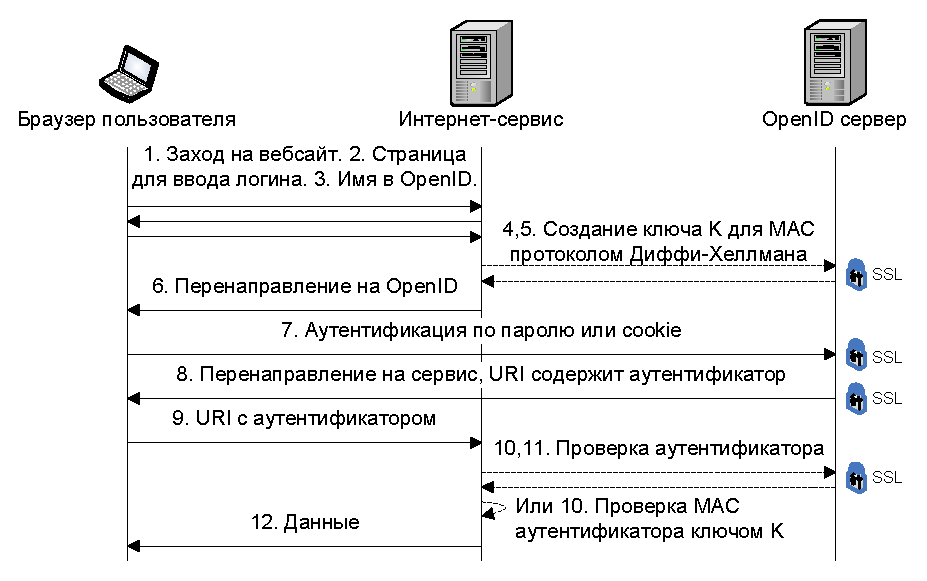
\includegraphics[width=0.9\textwidth]{pic/openid}
	\caption{Схема аутентификации в OpenID\label{fig:openid}}
\end{figure}

На рис.~\ref{fig:openid} показана схема аутентификации в OpenID версии 2 для доступа к стороннему интернет-сервису.

Если сервис и центр вместе создают общий секретный ключ $K$ для имитовставки\index{имитовставка} $\MAC_K$, выполняются шаги 4, 5 по протоколу Диффи~---~Хеллмана\index{протокол!Диффи~---~Хеллмана}:
\[ \begin{array}{l}
    \text{4. Сервис} ~\rightarrow~ \text{центр: модуль}~ p ~\text{группы}~ \Z_p^*, ~\text{генератор}~ g, \\
        ~~~~~~~~~~~~~~~\text{число}~ g^a \mod p, \\
    \text{5. Сервис} ~\leftarrow~ \text{центр: число}~ g^b \mod p, ~\text{гаммированный} \\
        ~~~~~~~~~~~~~~~\text{ключ}~ K \oplus (g^{ab} \mod p),
\end{array} \]
то аутентификатор содержит $\MAC_K$, проверяемый шагом 10 на выданном ключе $K$\footnote{Более правильным подходом является использование в качестве ключа $K = g^{ab} \mod p$, так как в этом случае ключ создаётся совместно, а не выдаётся центром.}. Имитовставка\index{имитовставка} определяется как описанный ранее $\HMAC$ с хэш-функцией SHA-256.

Если сервис и центр не создают общий ключ (этапы 4, 5 не выполняются), то сервис делает запрос на проверку аутентификатора в шагах 10, 11.

В OpenID аутентификатор состоит из следующих основных полей: имени пользователя, URL сервиса, результата аутентификации в OpenID, одноразовой метки и, возможно, кода аутентификации от полей аутентификатора на секретном ключе $K$, если он был создан на этапах 4, 5. Одноразовая метка является \emph{одноразовым} псевдослучайным идентификатором результата аутентификации, который центр сохраняет в своей БД. По одноразовой метке сервис запрашивает центр о верности результата аутентификации на этапах 10, 11. Одноразовая метка дополнительно защищает от атак воспроизведения.

Можно было бы исключить шаги 4, 5, 10, 11, но тогда сервису пришлось бы реализовывать и хранить в БД использованные одноразовые метки для защиты от атак воспроизведения. Цель OpenID -- предоставить аутентификацию с минимальными издержками на интеграцию. Поэтому в OpenID реализуется модель, в которой сервис делегирует все проверки центру с помощью соответствующих запросов.

Важно отметить, что в аутентификации через OpenID необходимо использовать TLS-соединения\index{протокол!SSL/TLS} (то есть протокол HTTPS\index{протокол!HTTPS}) при всех взаимодействиях с центром, так как в самом протоколе OpenID не производится аутентификация сервиса и центра, конфиденциальность\index{конфиденциальность} и целостность\index{целостность} не поддерживаются.


\subsection{Вторичная аутентификация по cookie}
\selectlanguage{russian}

Если сервер использует первичную аутентификацию по паролю, который передаётся в виде данных POST-запроса, то осуществлять подобную передачу данных при каждом обращении неудобно. Клиент должен иметь возможность доказать серверу, что он уже прошёл первичную аутентификацию. Должен быть предусмотрен механизм вторичной аутентификации. Для этого используется случайный токен, который уникален для каждого пользователя (обычно -- для каждого сеанса работы пользователя), который сервер передаёт пользователю после первичной аутентификации. Данный токен должен передаваться клиентом на сервис при каждом обращении к страницам, которые относятся к защищённой области сервиса. На практике применяются следующие механизмы для передачи данного токена при каждом запросе.

\begin{itemize}
	\item Первым способом является модификация вывода страницы клиенту, которая добавляет ко всем URL в HTML-коде страницы этот токен. В результате, переходя по ссылкам на HTML-странице (а также заполняя формы и отправляя их на сервер), клиент будет автоматически отправлять токен как часть запроса в URL-адресе страницы:

\texttt{http://tempuri.org/page.html?token=12345.}
	\item Вторым способом является использование механизма cookie (<<куки>>, <<кукиз>>, на русский обычно не переводится, подробнее см.~\cite[Client Identification and Cookies]{Totty:2002}). Данный механизм позволяет серверу передать пользователю некоторую строку, которая будет отправляться на сервер при каждом последующем запросе.
\end{itemize}

Основным механизмом для вторичной аутентификации пользователей в веб-сервисах является механизм cookie, а токены, как часть URL, используются в распределённых системах, наподобие уже рассмотренной OpenID, так как сервисы, находящиеся в разных доменах, не имеют доступа к общим cookie. Далее рассмотрим подробнее механизм использования cookie.

Когда браузер в первый раз делает HTTP-запрос:
\begin{center} \begin{verbatim}
GET /index.html HTTP/1.1
Host: www.wikipedia.org
Accept: */*
\end{verbatim} \end{center}

В заголовок ответа сервера веб-приложение может добавить заголовок \texttt{Set-Cookie}, который содержит новые значения cookie:
\begin{center} \begin{verbatim}
HTTP/1.1 200 OK
Content-type: text/html
Set-Cookie: name1=value1; name2=value2; ...

...далее HTML-страница...
\end{verbatim} \end{center}

Браузер, если это разрешено настройками, при последующих запросах к веб-серверу автоматически будет отсылать cookie назад веб-приложению:
\begin{center} \begin{verbatim}
GET /wiki/HTTP_cookie HTTP/1.1
Host: www.wikipedia.org
Cookie: name1=value1; name2=value2; ...
Accept: */*
\end{verbatim} \end{center}

Далее веб-приложение может создать новый cookie, изменить значение старого и~т.\,д. Браузер хранит cookie на устройстве клиента. То есть cookie позволяет хранить переменные на устройстве клиента, отсылать сохранённые значения, получать новые переменные. В результате создаётся передача состояний, что даёт возможность не вводить логин и пароль каждый раз при входе в интернет-сервис, использовать несколько окон для одного сеанса работы в интернет-магазине и~т.\,д. При создании cookie может указываться его конечное время действия, после которого браузер удалит устаревший cookie.

Для вторичной аутентификации в cookie веб-приложение записывает токен в виде текстовой строки. В качестве токена можно использовать \emph{псевдослучайную} текстовую строку достаточной длины, созданную веб-приложением. Например:
\begin{center} \begin{verbatim}
Cookie: auth=B35NMVNASUY26MMWNVZ87.
\end{verbatim} \end{center}

В этом случае веб-сервис должен вести журнал выданных токенов пользователям и их сроков действия. Если информационная система небольшого размера (один или десятки серверов), то вместо журнала может использоваться механизм session storage.
\begin{itemize}
	\item При первом заходе на сайт сервер приложений (платформа исполнения веб-приложения) <<назначает>> клиенту сессию, отправляя ему через механизм cookie новый (псевдо)случайный токен сессии, а в памяти сервера выделяя структуру, которая недоступна самому клиенту, но которая соответствует данной конкретной сессии.
	\item При каждом последующем обращении клиент передаёт токен (идентификатор) сессии с помощью механизма cookie. Сервер приложений берёт из памяти соответствующую структуру сессии и передаёт её приложению вместе с параметрами запроса.
	\item В момент прохождения первичной аутентификации приложение добавляет в указанную область памяти ссылку на информацию о пользователе.
	\item При последующих обращениях приложение использует информацию о пользователе, записанную в области памяти сессии клиента.
	\item Сессия автоматически стирается из памяти после прохождения некоторого времени неактивности клиента (что контролируется настройками сервера) либо если приложение явно вызвало функцию инвалидации сессии (\langen{invalidate}).
\end{itemize}

Плюсом использования session storage является то, что этот механизм уже реализован в большинстве платформ для построения веб-приложений (см., например, \cite[Controlling sessions]{Brittain:Darwin:2007}). Его минусом является сложность синхронизации структур сессий в памяти серверов для распределённых информационных систем большого размера.

Вторым способом вторичной аутентификации с использованием cookie является непосредственное включение аутентификационных данных (идентификатор пользователя, срок действия) в cookie вместо случайного токена. К данным в обязательном порядке добавляется имитовставка\index{имитовставка} по ключу, который известен только сервису. С одной стороны, данный подход может значительно увеличить размер передаваемых cookie. С другой -- он облегчает вторичную аутентификацию в распределённых системах, так как промежуточным сервисом, хранящим информацию о произошедшей аутентификации, является только клиент, а не сервер.

Конечно, беспокоиться об аутентификации в веб-сервисах при использовании обычного HTTP-протокола\index{протокол!HTTP} без зашифрованного SSL-соединения\index{протокол!SSL/TLS} имеет смысл только по отношению к угадыванию токенов аутентификации другими пользователями, которые не имеют доступа к маршрутизаторам и сети, через которые клиент общается с сервисом. Кража компьютера или одного cookie-файла и перехват незащищённого трафика протокола HTTP\index{протокол!HTTP} приводят к доступу в систему под именем взломанного пользователя.


